\documentclass[border=4pt,12pt]{standalone}
% House style for redrawn exam diagrams (diagram-v4: 0.4pt lines, filled -latex arrows, fine dashes; stipple and hatching drawn as real dots/lines (no PDF/SVG patterns, so they render in every browser and at any scale); transparent background). Every figure \input's this.
\usepackage{amsmath,amssymb}
\usepackage{txfonts}
\usepackage{pdfrender,xcolor}
% \halo{text}: label on shading. The shading stops just around each letter's outline (a thin knock-out that follows the
% glyphs, like the papers' typesetting), never a box. Owner: "I don't want a box around the text".
\newcommand{\halo}[1]{\leavevmode\rlap{\pdfrender{TextRenderingMode=2,LineWidth=2.2pt,LineJoinStyle=1,StrokeColor=white,FillColor=white}#1}#1}
\usepackage{tikz,pgfplots}
\pgfplotsset{compat=1.18}
\usetikzlibrary{arrows.meta,calc,angles,quotes,patterns,patterns.meta,intersections,positioning,decorations.markings,shapes.geometric}
% Stipple and hatching are drawn as actual dots / lines clipped to the region (path picture), NOT as pattern fills:
% SVG <pattern> fills vanish or blur when browsers scale the image, so the owner could not see the shading.
% Each dot is a 0.72pt square (keeps SVGs small; reads as a dot at print size). Dots sit on one global staggered grid, so neighbouring regions line up.
\makeatletter
\newdimen\ex@x \newdimen\ex@y \newdimen\ex@xa \newdimen\ex@ya \newdimen\ex@xb \newdimen\ex@yb \newcount\ex@row
\def\exam@stipplecolor{black!75}\def\exam@dotr{0.42pt}\def\exam@dotgap{2.5}
\def\ex@rowdots{\ifdim\ex@x<\ex@xb \pgfpathrectangle{\pgfqpoint{\dimexpr\ex@x-0.36pt\relax}{\dimexpr\ex@y-0.36pt\relax}}{\pgfqpoint{0.72pt}{0.72pt}}\advance\ex@x by \exam@dotgap pt\relax\expandafter\ex@rowdots\fi}
\def\exam@stipple{%
  \pgftransformreset% dots are sized in real points even inside scaled pictures
  \pgfpointanchor{path picture bounding box}{south west}\ex@xa=\pgf@x \ex@ya=\pgf@y
  \pgfpointanchor{path picture bounding box}{north east}\ex@xb=\pgf@x \ex@yb=\pgf@y
  \pgfsetfillcolor{\exam@stipplecolor}\pgfmathsetmacro\ex@h{\exam@dotgap/2}%
  \pgfmathtruncatemacro\ex@r{floor(\ex@ya/\ex@h)-1}\ex@row=\ex@r\relax
  \ex@y=\ex@r\dimexpr\ex@h pt\relax
  \loop\ifdim\ex@y<\ex@yb
    \pgfmathtruncatemacro\ex@c{floor(\ex@xa/\exam@dotgap)-1}\ex@x=\ex@c\dimexpr\exam@dotgap pt\relax
    \ifodd\ex@row \advance\ex@x by \ex@h pt\fi
    \ex@rowdots
    \advance\ex@y by \ex@h pt \advance\ex@row by 1
    \ifnum\numexpr\ex@row-(\ex@row/4)*4\relax=0 \pgfusepath{fill}\fi% flush every 4 rows: bounded TeX memory, few clip copies in the SVG
  \repeat\pgfusepath{fill}}
\newdimen\ex@d
\def\exam@hatch#1{% #1 = 1 for /, -1 for \ ; lines 45 degrees, 3pt apart
  \pgftransformreset
  \pgfpointanchor{path picture bounding box}{south west}\ex@xa=\pgf@x \ex@ya=\pgf@y
  \pgfpointanchor{path picture bounding box}{north east}\ex@xb=\pgf@x \ex@yb=\pgf@y
  \ex@d=\dimexpr\ex@yb-\ex@ya\relax \ex@x=\dimexpr\ex@xa-\ex@d\relax
  \loop\ifdim\ex@x<\ex@xb
    \ifnum#1>0 \pgfpathmoveto{\pgfqpoint{\ex@x}{\ex@ya}}\pgfpathlineto{\pgfqpoint{\dimexpr\ex@x+\ex@d\relax}{\ex@yb}}%
    \else \pgfpathmoveto{\pgfqpoint{\ex@x}{\ex@yb}}\pgfpathlineto{\pgfqpoint{\dimexpr\ex@x+\ex@d\relax}{\ex@ya}}\fi
    \advance\ex@x by 4.24pt
  \repeat
  \pgfsetlinewidth{0.4pt}\pgfsetstrokecolor{black}\pgfusepath{stroke}}
\def\examstipple{\exam@stipple}\def\examhatch{\exam@hatch}\def\examsetstipplecolor#1{\def\exam@stipplecolor{#1}}\def\examsetdotgap#1{\def\exam@dotgap{#1}}
\makeatother
% (legacy pattern kept for old files)
% staggered stipple like the NESA papers' dotted shading
\pgfdeclarepatternformonly{exam stipple}{\pgfpointorigin}{\pgfqpoint{2.2pt}{2.2pt}}{\pgfqpoint{2.2pt}{2.2pt}}{%
  \pgfpathcircle{\pgfqpoint{0.55pt}{0.55pt}}{0.42pt}\pgfpathcircle{\pgfqpoint{1.65pt}{1.65pt}}{0.42pt}\pgfusepath{fill}}
\tikzset{
  every picture/.style={line width=0.6pt, >={Latex[length=2mm,width=1.3mm]}},
  curve/.style={line width=0.6pt},
  open arrow/.style={-{Latex[length=2mm,width=1.3mm]}},  % owner: filled -latex heads everywhere, no open chevrons
  aux/.style={dash pattern=on 2pt off 1.5pt, line width=0.6pt},
  shade/.code={\def\exA{#1}\def\exB{none}\ifx\exA\exB\else\pgfkeysalso{fill=black!18}\fi},
  shade/.default=on,
  shade dots/.style={fill=none, path picture={\examstipple}},
  stipple color/.code={\examsetstipplecolor{#1}},
  stipple gap/.code={\examsetdotgap{#1}},
  shade dense dots/.style={fill=none, stipple gap=1.6, path picture={\examstipple}},
  shade hatch/.style={fill=none, path picture={\examhatch{1}}},
  shade hatch reverse/.style={fill=none, path picture={\examhatch{-1}}},
  shade solid/.style={fill=black},
  pt/.style={circle, fill, inner sep=1.1pt},
  open pt/.style={circle, draw, fill=white, inner sep=1.1pt},
}
\pgfplotsset{
  exam axes/.style={axis lines=middle, axis line style={->}, xlabel={$x$}, ylabel={$y$},
    xlabel style={anchor=west}, ylabel style={anchor=south}, tick label style={font=\small},
    every axis plot/.append style={line width=0.6pt, black}, samples=200, clip=false,
    enlargelimits=false, axis on top},
}

\begin{document}
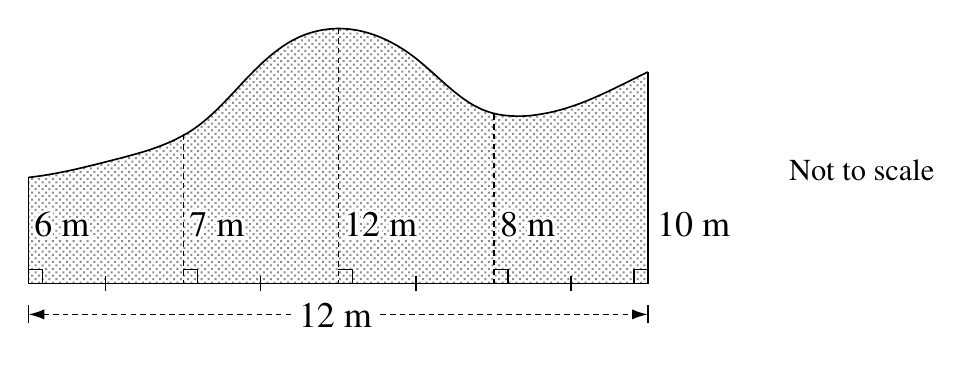
\begin{tikzpicture}[x=0.0127cm,y=-0.0127cm,every node/.style={font=\fontsize{13}{15}\selectfont}]
\path[shade dots, stipple color=black!45] plot[smooth] coordinates {(69,182) (81.98,180.3) (95.08,178.1) (108.4,175.5) (121.7,172.5) (135.3,169.2) (149.2,165.7) (163.2,162.1) (176.4,158.5) (188.8,154.8) (200.4,150.7) (211.4,146.2) (221.5,141.2) (230.9,135.8) (239.7,129.6) (248.5,122.4) (257.5,114.1) (266.6,104.9) (276.3,94.65) (286,84.22) (295.3,74.71) (304.3,66.05) (313.4,58.25) (322.2,51.63) (331,46.05) (340,41.47) (348.9,38) (358.3,35.39) (367.9,33.74) (377.7,33.05) (387.3,33.36) (397.2,34.65) (407,36.92) (417,40.19) (426.8,44.35) (436.5,49.39) (446,55.27) (455.3,61.95) (464.7,69.67) (474.9,78.6) (485.5,88.16) (495.2,96.4) (504.3,103.4) (513,109) (521.4,113.4) (529.8,116.6) (538.7,118.9) (548.3,120.2) (558.4,120.7) (569.1,120.3) (580.1,118.9) (591.4,116.8) (602.9,113.9) (614.5,110.2) (626.2,105.9) (637.9,100.9) (650.2,95.28) (662.7,89.21) (675.8,82.72) (688.5,76.5)} -- (688.5,288) -- (69,288) -- cycle;
\draw plot[smooth] coordinates {(69,182) (81.98,180.3) (95.08,178.1) (108.4,175.5) (121.7,172.5) (135.3,169.2) (149.2,165.7) (163.2,162.1) (176.4,158.5) (188.8,154.8) (200.4,150.7) (211.4,146.2) (221.5,141.2) (230.9,135.8) (239.7,129.6) (248.5,122.4) (257.5,114.1) (266.6,104.9) (276.3,94.65) (286,84.22) (295.3,74.71) (304.3,66.05) (313.4,58.25) (322.2,51.63) (331,46.05) (340,41.47) (348.9,38) (358.3,35.39) (367.9,33.74) (377.7,33.05) (387.3,33.36) (397.2,34.65) (407,36.92) (417,40.19) (426.8,44.35) (436.5,49.39) (446,55.27) (455.3,61.95) (464.7,69.67) (474.9,78.6) (485.5,88.16) (495.2,96.4) (504.3,103.4) (513,109) (521.4,113.4) (529.8,116.6) (538.7,118.9) (548.3,120.2) (558.4,120.7) (569.1,120.3) (580.1,118.9) (591.4,116.8) (602.9,113.9) (614.5,110.2) (626.2,105.9) (637.9,100.9) (650.2,95.28) (662.7,89.21) (675.8,82.72) (688.5,76.5)};
\draw (69,182) -- (69,288) -- (688.5,288) -- (688.5,76.5);
\foreach \x/\t in {224/139,379/33,535/119} \draw[aux] (\x,\t) -- (\x,288);
\foreach \x in {146,301,456.5,611.5} \draw (\x,281) -- (\x,296);
\foreach \x in {69,224,379,535} \draw (\x,274) -- (\x+14,274) -- (\x+14,288);
\draw (688.5,274) -- (674.5,274) -- (674.5,288);
\draw (69,310) -- (69,328); \draw (688.5,310) -- (688.5,328);
\draw[aux,<-] (69,319) -- (332,319); \draw[aux,->] (421,319) -- (688.5,319);
\node at (376,320) {12 m};
\node[anchor=west,inner sep=0] at (74,229) {\halo{6 m}};
\node[anchor=west,inner sep=0] at (229,229) {\halo{7 m}};
\node[anchor=west,inner sep=0] at (384,229) {\halo{12 m}};
\node[anchor=west,inner sep=0] at (540,229) {\halo{8 m}};
\node[anchor=west,inner sep=0] at (697,229) {10 m};
\node[anchor=west,inner sep=0,font=\fontsize{11}{13}\selectfont] at (829,175) {Not to scale};
\end{tikzpicture}
\end{document}
